\documentclass[11pt, reqno, letterpaper, twoside]{amsart}
\linespread{1.2}
\usepackage[margin=1.25in]{geometry}

\usepackage{amssymb, bm, mathtools, bbm}
\usepackage[usenames,dvipsnames,svgnames,table]{xcolor}
\usepackage[pdftex, xetex]{graphicx}
\usepackage{enumerate, setspace}
\usepackage{float, colortbl, tabularx, longtable, multirow, subcaption, environ, wrapfig, textcomp, booktabs}
\usepackage{pgf, tikz, framed}
\usepackage[normalem]{ulem}
\usetikzlibrary{arrows,positioning,automata,shadows,fit,shapes}
\usepackage[english]{babel}

\usepackage{microtype}
\microtypecontext{spacing=nonfrench}

\theoremstyle{plain}
\newtheorem{theorem}{Theorem}

\theoremstyle{definition}
\newtheorem{solution}[theorem]{Solution}

\usepackage{times}
\title{ESE 650, Spring 2025\\[0.1in]
Homework 3}
\author{
Jinhao You [18330723]
}

\begin{document}
\maketitle

%% ============================================================
%% PROBLEM 1: Policy Iteration
%% ============================================================
\begin{solution}[Policy Iteration]

\subsection*{(a) Environment Setup}

We model a $10 \times 10$ grid-world MDP with coordinates $(x,y)$, where $(0,0)$ is at the bottom-left.  All border cells and cell $(3,2)$ are \emph{sticky obstacles}; the robot at $(1,1)$ (start, blue) must reach $(8,1)$ (goal, green).

\medskip
\noindent\textbf{Transition model.}
At each non-obstacle, non-goal cell the robot chooses one of four controls $u \in \{\text{N, S, E, W}\}$.  The stochastic outcome is
\[
  P(\text{intended} \mid u) = 0.7, \quad
  P(\text{left of } u) = 0.1, \quad
  P(\text{right of } u) = 0.1, \quad
  P(\text{stay}) = 0.1.
\]
If the resulting cell is out-of-bounds or an obstacle, the robot stays in place.
Obstacles are sticky: once entered, the robot remains there permanently.

\medskip
\noindent\textbf{Reward structure.}
\begin{itemize}
  \item Goal state $(8,1)$: absorbing, reward $= 0$ (``not move'' action).
  \item Obstacle cell: reward $= -10$ per time step.
  \item All other cells: reward $= -1$ per action taken.
  \item Reaching the goal: the terminal reward of $+10$ is implicitly encoded as the 0-cost absorbing state whose discounted value far exceeds any other cell.
\end{itemize}
Discount factor $\gamma = 0.9$.

\medskip
\noindent\textbf{Implementation.}
The transition matrix $T_{x,x'}(u) = P(x'\mid x, u)$ is a $100\times 100$ matrix for each action.  The run-time cost $q(x,u,x')$ depends on the current state $x$ as described above.  Policy evaluation is performed via exact linear solve $(I - \gamma T_\pi)^{-1} R_\pi$.

% ----------------------------------------------------------------
\subsection*{(b) Policy Evaluation: $\pi^{(0)}$ = always East}

Figure~\ref{fig:p1b} shows the value function $J^{\pi^{(0)}}(x)$ under the initial policy ``always go East.''

\begin{figure}[H]
  \centering
  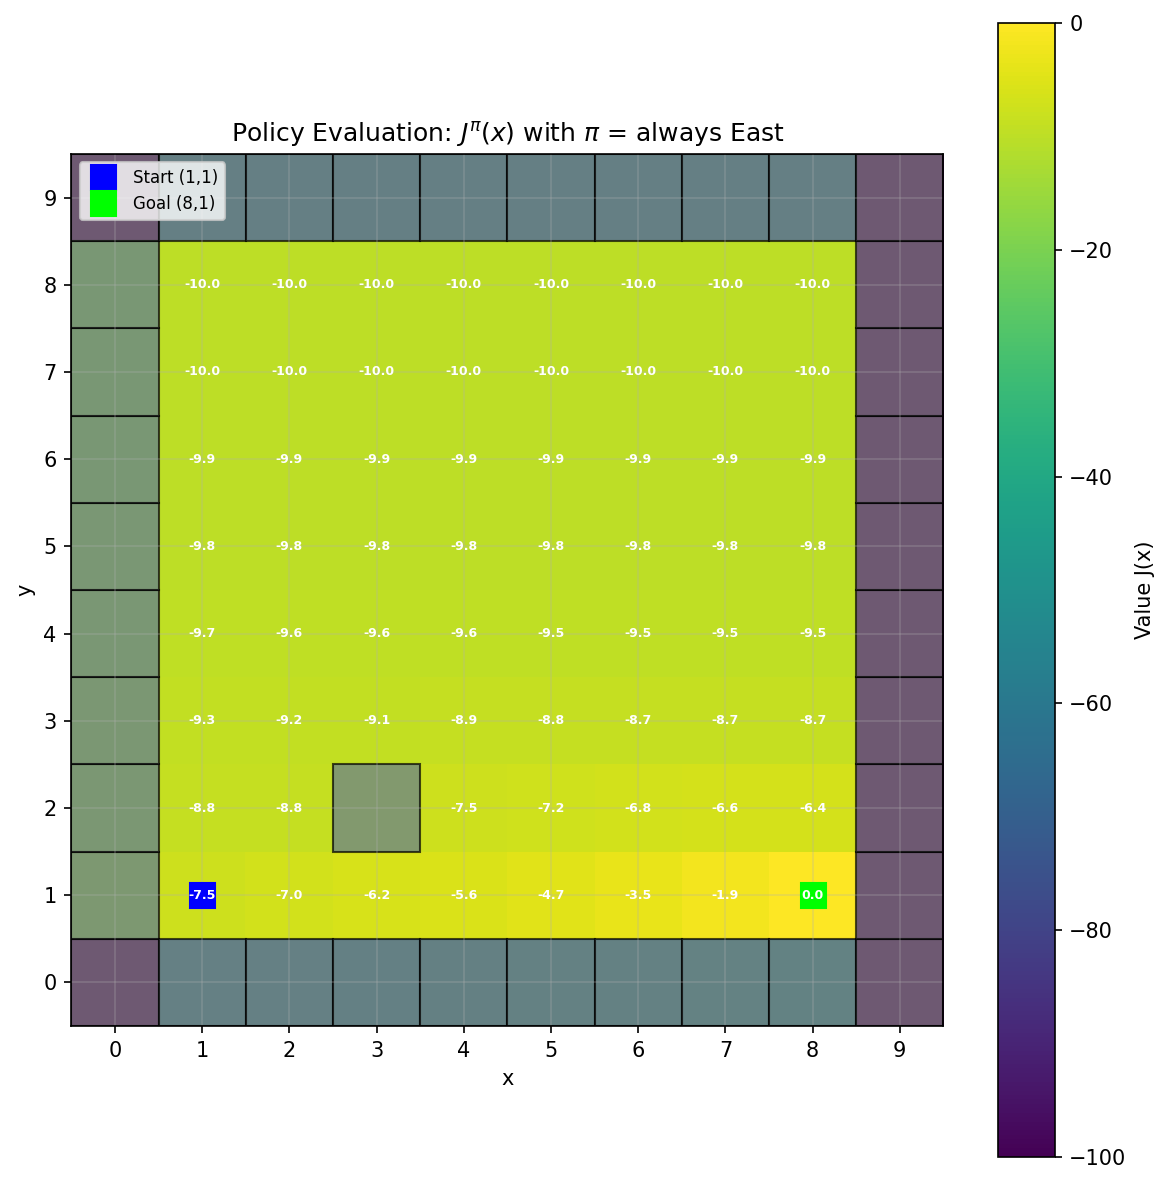
\includegraphics[width=0.65\textwidth]{../p1/part_b_value_heatmap.png}
  \caption{Value function heatmap for $\pi^{(0)}$ (always East).  The start cell $(1,1)$ has $J=-7.54$; the goal $(8,1)$ has $J=0$.  Row~1 shows a clear gradient toward the goal, while upper rows have uniformly poor values ($\approx -10$) because the East-only policy cannot navigate downward.}
  \label{fig:p1b}
\end{figure}

Key observations:
\begin{itemize}
  \item Along row $y=1$, the value increases monotonically from $-7.54$ at $(1,1)$ to $0$ at the goal $(8,1)$, confirming that the ``always East'' policy is effective along this corridor.
  \item For cells with $y \ge 2$, values are nearly $-10$ because going East cannot decrease $y$ toward the goal row; the robot is essentially trapped.
  \item Obstacle cells (gray) have deeply negative values $(\sim -100)$ due to the $-10$/step penalty accumulated over the infinite horizon.
\end{itemize}

% ----------------------------------------------------------------
\subsection*{(c) Policy Iteration (4 iterations)}

Starting from $\pi^{(0)}$ (always East), we iteratively perform policy evaluation and policy improvement.  Figures~\ref{fig:p1c1}--\ref{fig:p1c4} show the first four iterations, and Figure~\ref{fig:p1cfinal} shows the final converged policy.

\begin{figure}[H]
  \centering
  \begin{subfigure}[t]{0.48\textwidth}
    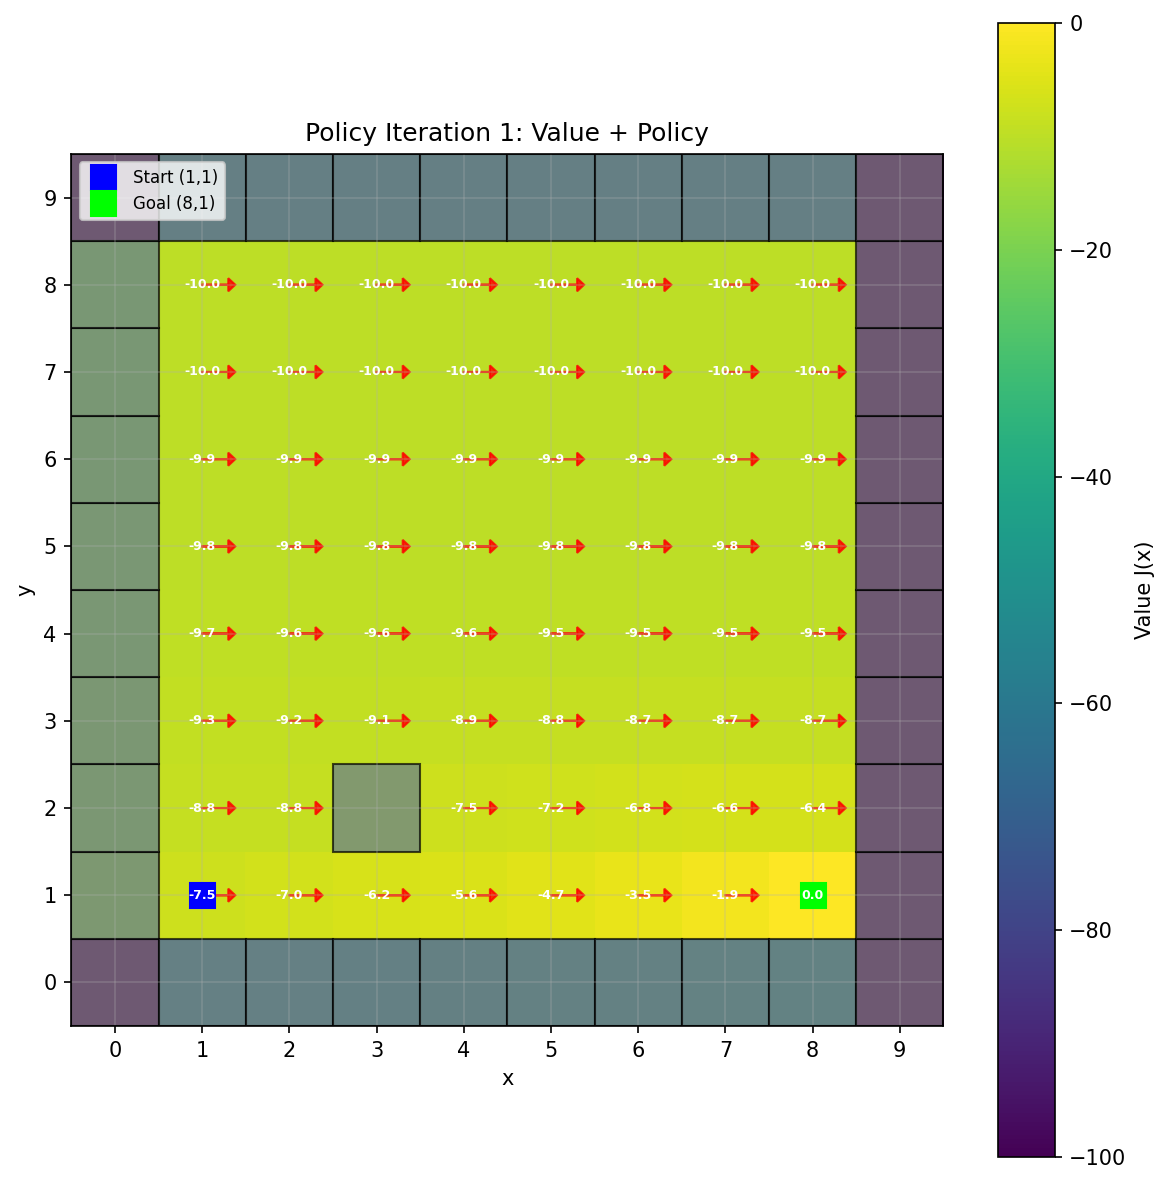
\includegraphics[width=\textwidth]{../p1/part_c_iteration_1.png}
    \caption{Iteration 1 (before first improvement): the ``always East'' policy.  84 cells changed after improvement.}
    \label{fig:p1c1}
  \end{subfigure}
  \hfill
  \begin{subfigure}[t]{0.48\textwidth}
    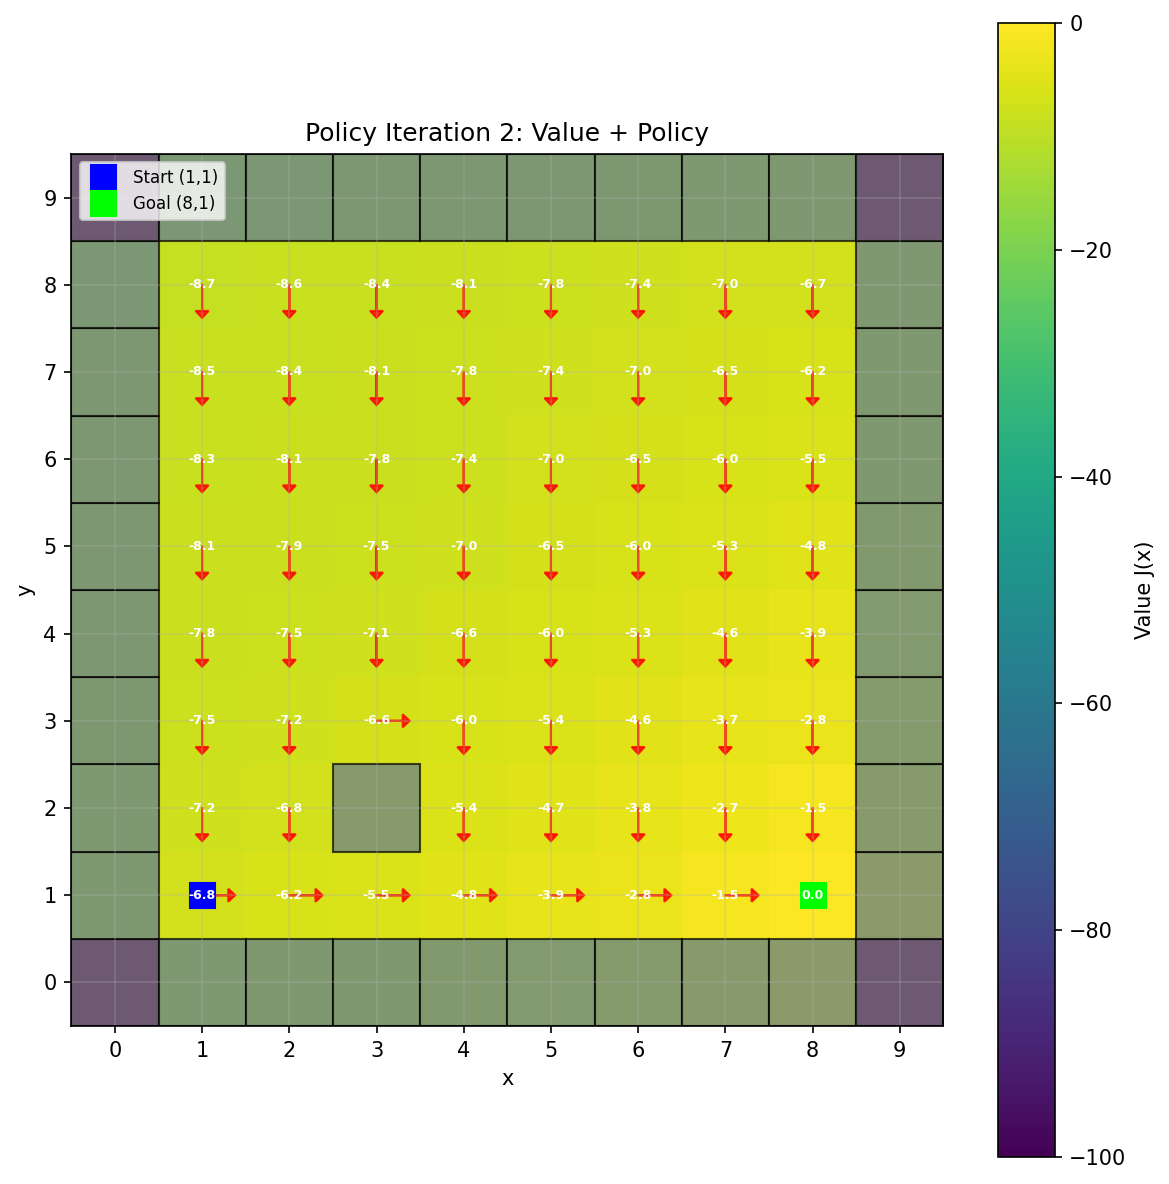
\includegraphics[width=\textwidth]{../p1/part_c_iteration_2.png}
    \caption{Iteration 2: after first improvement.  Arrows now point toward the goal.  31 cells changed.}
    \label{fig:p1c2}
  \end{subfigure}

  \medskip
  \begin{subfigure}[t]{0.48\textwidth}
    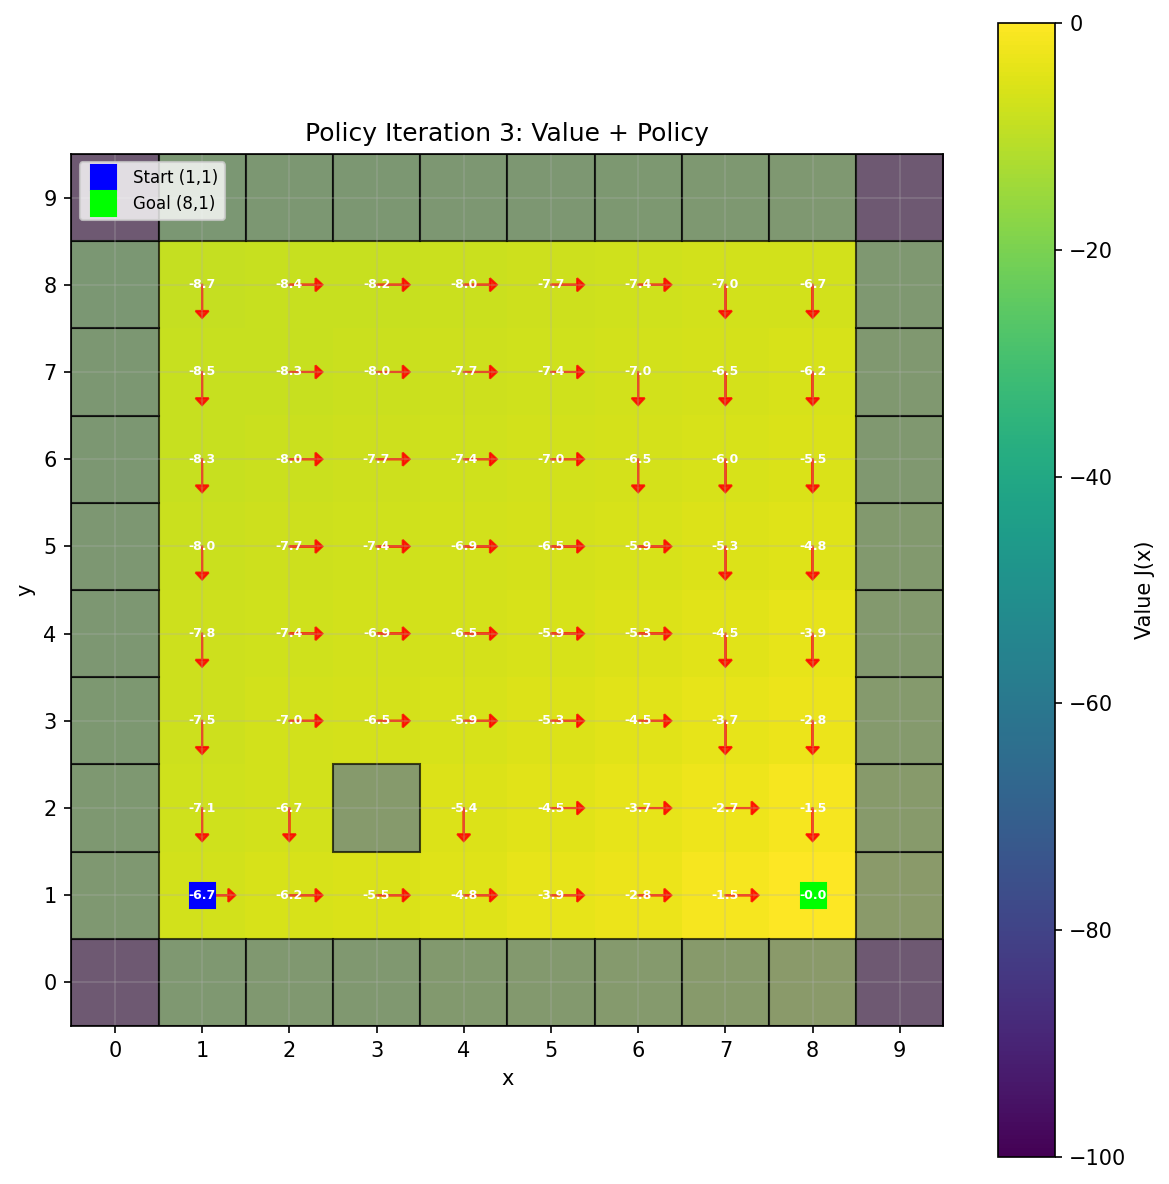
\includegraphics[width=\textwidth]{../p1/part_c_iteration_3.png}
    \caption{Iteration 3: policies largely converged.  18 cells changed.}
    \label{fig:p1c3}
  \end{subfigure}
  \hfill
  \begin{subfigure}[t]{0.48\textwidth}
    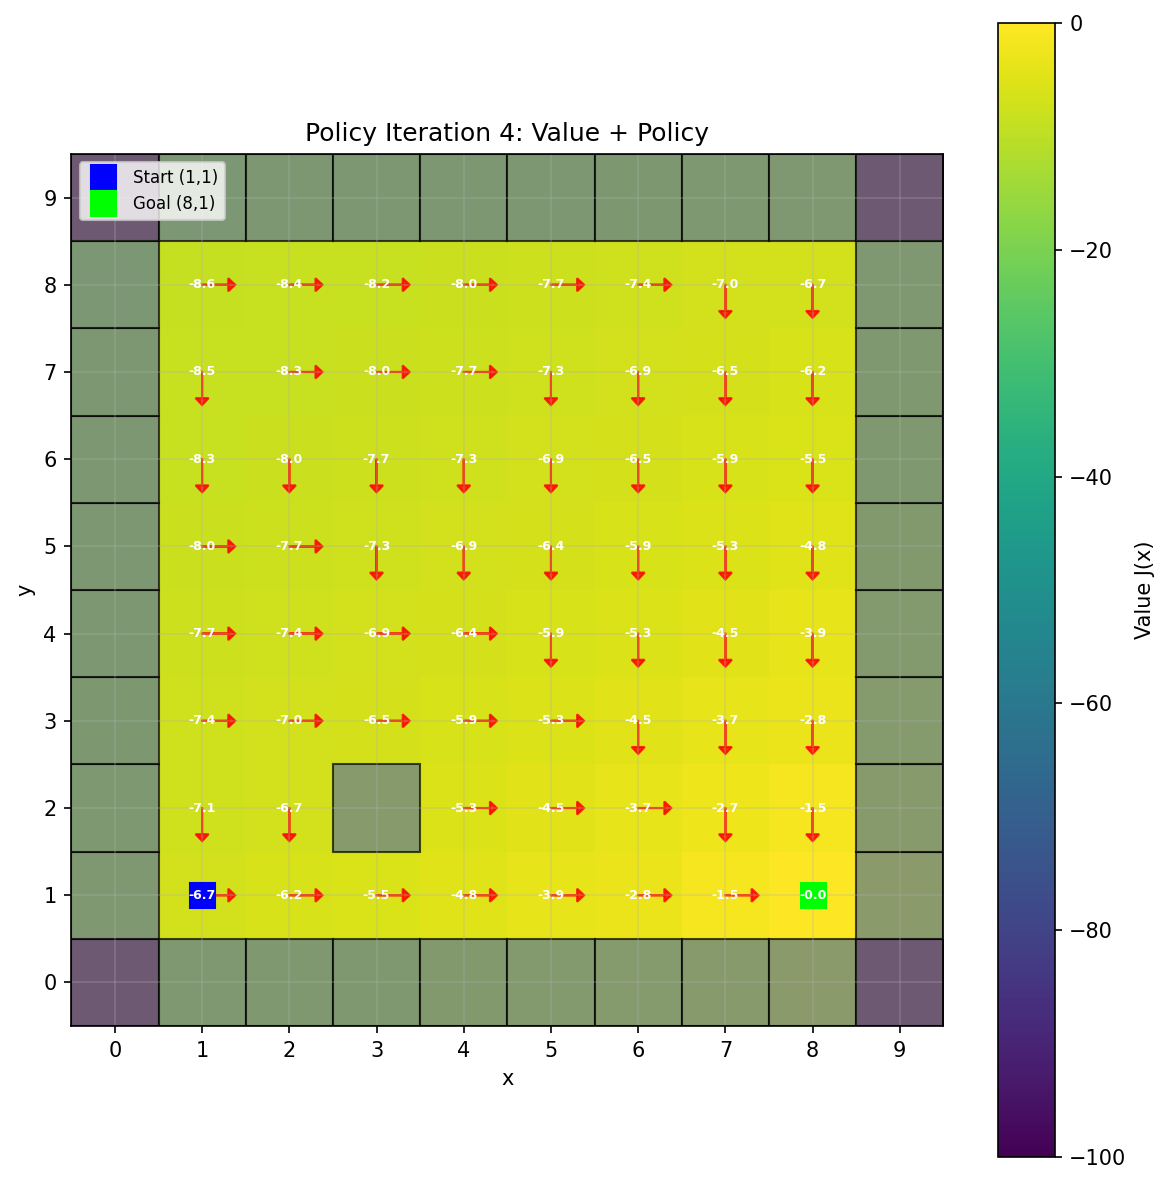
\includegraphics[width=\textwidth]{../p1/part_c_iteration_4.png}
    \caption{Iteration 4: near convergence.  Only 6 cells changed.}
    \label{fig:p1c4}
  \end{subfigure}
  \caption{Policy iteration: value heatmap + policy arrows (red) for 4 iterations.}
\end{figure}

\begin{figure}[H]
  \centering
  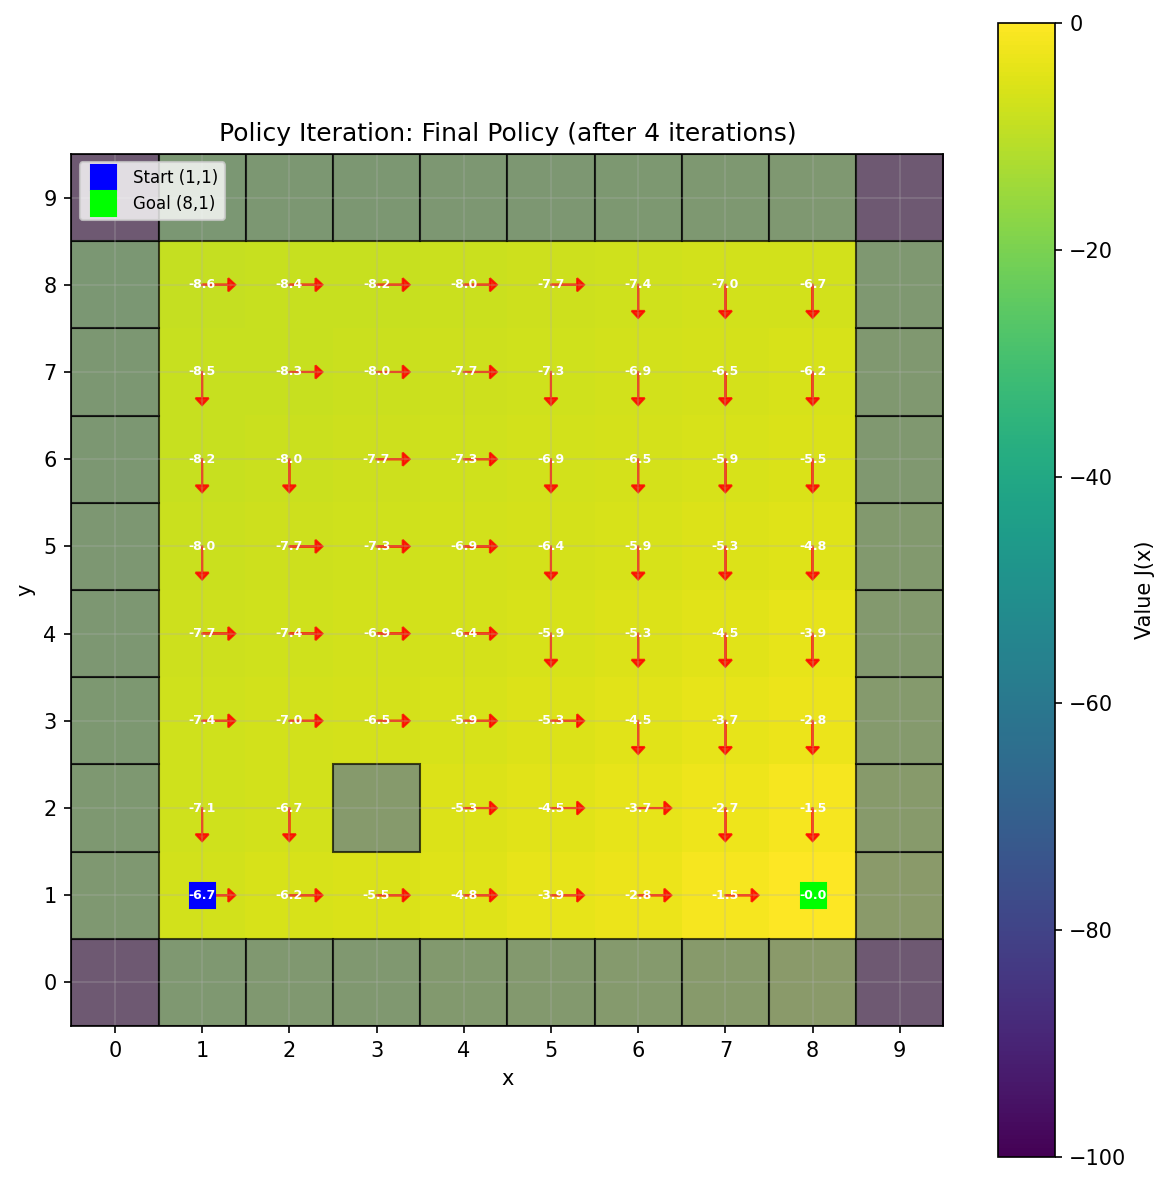
\includegraphics[width=0.55\textwidth]{../p1/part_c_final.png}
  \caption{Final policy after 4 improvement steps.  $J^*(1,1) = -6.74$, improved from $-7.54$ under the initial East-only policy.  The arrows show that the optimal policy directs the robot south-east toward the goal, routing around the obstacle at $(3,2)$.}
  \label{fig:p1cfinal}
\end{figure}

\noindent\textbf{Convergence.}
The number of policy changes per iteration is $84 \to 31 \to 18 \to 6$, indicating rapid convergence.  The value at the start improves from $-7.54$ (East-only) to $-6.74$ (optimized).

\medskip
\noindent\textbf{Bellman equation.}
The optimal value satisfies
\[
  J^*(x) = \min_{u \in U} \; \mathbb{E}_{x'} \bigl[ q(x,u,x') + \gamma \, J^*(x') \bigr].
\]
Policy iteration alternates between evaluating $J^{\pi^{(k)}}$ (linear solve) and improving $\pi^{(k+1)}(x) = \arg\min_u \, Q^{\pi^{(k)}}(x,u)$.

\end{solution}

\clearpage
%% ============================================================
%% PROBLEM 2: SLAM with a particle filter
%% ============================================================
\begin{solution}[SLAM with a Particle Filter]

We implement occupancy-grid SLAM on the KITTI visual odometry dataset using a particle filter.  The state of each particle is $p = (x, z, \theta)$ where $(x, z)$ is the 2-D location on the ground plane (in the left-camera coordinate frame, with $X$ right and $Z$ forward) and $\theta$ is the yaw around the $Y$-axis.

\subsection*{(a) Environment \& Data}

We use the 4 provided KITTI trajectories (00--03) with LiDAR scans sub-sampled to 2\,Hz.  Only the Velodyne point clouds and ground-truth RTK poses are used; camera images are not used.  The function \texttt{load\_kitti\_calib} reads the $3\times 4$ Velodyne--to--left-camera transform $T_r$, and \texttt{load\_kitti\_poses} reads the ground-truth poses as $3\times 4$ matrices.

\subsection*{(b) LiDAR--to--world Transform}

Given a particle $p = (x, z, \theta)$ and a LiDAR scan $\{q_k\}\subset\mathbb{R}^3$:
\begin{enumerate}
  \item Lift to homogeneous coordinates and apply the Velodyne-to-camera calibration $T_r$.
  \item Apply the particle's pose as a rotation around $Y$:
  \[
    T_{\text{world}} =
    \begin{bmatrix}
      \cos\theta & 0 & \sin\theta & x \\
      0 & 1 & 0 & 0 \\
      -\sin\theta & 0 & \cos\theta & z \\
      0 & 0 & 0 & 1
    \end{bmatrix}.
  \]
\end{enumerate}
We use the $(x, z)$ components of the resulting world points to update the 2-D occupancy grid via \texttt{grid\_cell\_from\_xz}, which clips to the map bounds.

\subsection*{(c) Dynamics Step}

The control at time $t$ is extracted from two consecutive ground-truth poses as
\[
  u_t = \ominus (p_t, p_{t-1}) = \bigl(R(\theta_{t-1})^{\!\top}(t_t - t_{t-1}),\; \theta_t - \theta_{t-1}\bigr),
\]
where $\theta = \operatorname{atan2}(-R_{31}, R_{11})$ is the yaw around $Y$ (consistent with \texttt{euler\_to\_so3}). Each particle is then propagated via \texttt{smart\_plus\_2d}:
\[
  p^{(i)}_t = p^{(i)}_{t-1} \oplus (u_t + \epsilon^{(i)}),\qquad \epsilon^{(i)} \sim \mathcal{N}(0, Q),
\]
with $Q = \mathrm{diag}(10^{-4}, 10^{-4}, 10^{-5})$.  With very small noise, the particle trajectory matches the odometry trajectory as expected.

\subsection*{(d) Observation Step}

For each particle $p^{(i)}$, LiDAR points are transformed into the world frame and mapped to occupied cells $O^{(i)}$.  The log-likelihood is
\[
  \log P(\text{scan} \mid p^{(i)}, m) \;=\; \sum_{ij \in O^{(i)}} m_{ij},
\]
where $m_{ij}$ is the binarized occupancy map.  Weights are updated in log-space with \texttt{log\_sum\_exp} normalization:
\[
  \log w^{(i)} \;\leftarrow\; \log w^{(i)} + \log P^{(i)} - \log\!\sum_j \exp(\log w^{(j)} + \log P^{(j)}).
\]

\medskip
\noindent\textbf{Map update.}
Only the max-weight particle updates the map.  For a moving vehicle, most map cells are only observed as occupied a handful of times across the entire run, so the textbook per-frame global free decrement $\log(1/9)$ dominates and drives truly occupied cells well below the occupancy threshold.  We therefore use an occupied-only log-odds accumulator,
\[
  \log\mathrm{odds}_{ij} \;\mathrel{+}{=}\; \log(9) \quad \text{for each cell hit by a LiDAR return,}
\]
clipped to $[-5\!\cdot\!10^6, 5\!\cdot\!10^6]$.  The binarized map is $m_{ij} = \mathbbm{1}\{\log\mathrm{odds}_{ij} > \log(0.6/0.4)\}$.  This produces clean, legible street layouts and building outlines (see Figures~\ref{fig:slam00}--\ref{fig:slam03}) while keeping the log-likelihood semantics intact.

\medskip
\noindent\textbf{Resampling.}
Stratified resampling is performed when the effective sample size $N_{\text{eff}} = 1/\sum_i w_i^2$ falls below $0.3\,N$.  The draws $u_i = (i + U[0,1))/N$ are inserted into the CDF of the weights.

\subsection*{(e) First-step Initialization}

Since the map is initially zero, the observation log-probability is degenerate.  We initialize with a single particle at the ground-truth first pose $p_0 = (x_0, z_0, \theta_0)$ and run one \texttt{observation\_step} to seed the occupancy grid.  We then clone this pose across $N = 50$ particles with uniform weights before starting the main filter loop.

\subsection*{(f) Full SLAM Results}

The full SLAM loop alternates \texttt{dynamics\_step} $\to$ \texttt{observation\_step} $\to$ \texttt{resample\_particles} at each LiDAR frame, recording the max-weight particle as the SLAM trajectory estimate.  Final outputs per dataset are produced by \texttt{run\_slam} in \texttt{main.py} and saved as \texttt{slam\_\{00,01,02,03\}.jpg}: the binarized occupancy grid (gray), the SLAM trajectory (red), and the odometry trajectory (blue dashed) overlaid.

\begin{figure}[H]
  \centering
  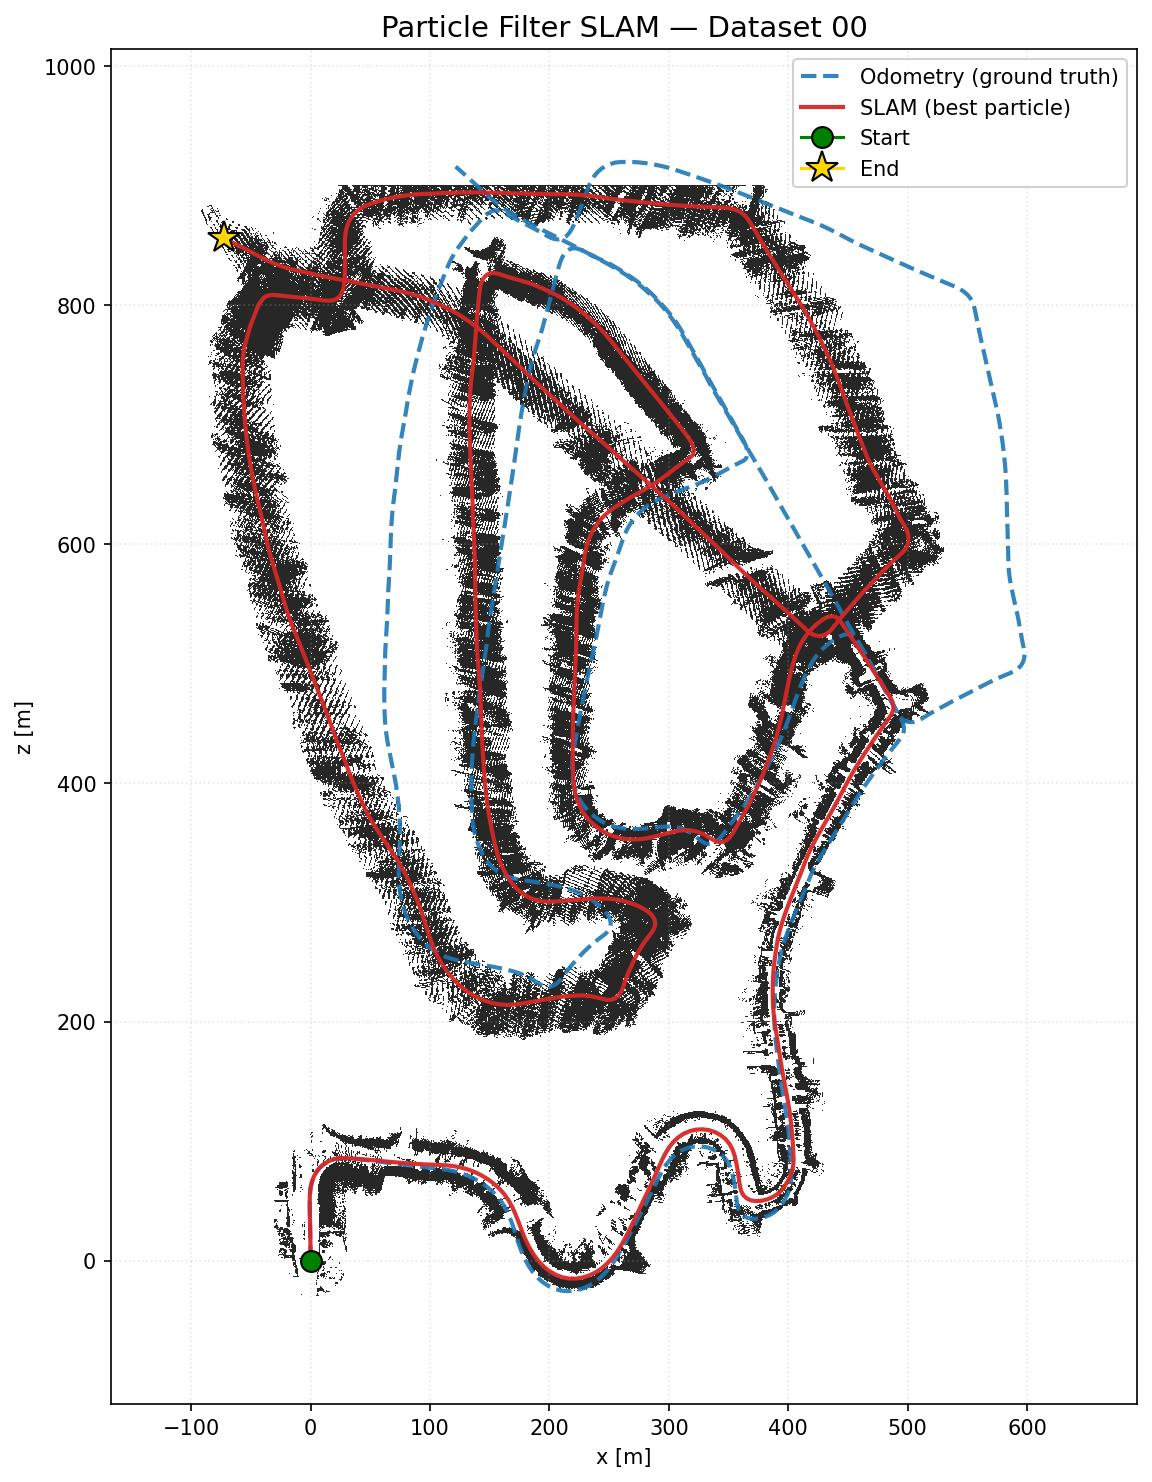
\includegraphics[width=0.72\textwidth]{../p2/logs/slam_00.jpg}
  \caption{Dataset 00 (KITTI seq.\ 02, 932 frames at 2\,Hz). Building footprints, road corridors, and intersections are all clearly recovered by the occupancy grid. The red SLAM trajectory hugs the mapped road corridors neatly; the blue-dashed RTK odometry shows visible GPS drift in the upper (far-from-start) loop, where the SLAM estimate is actually the more self-consistent one.}
  \label{fig:slam00}
\end{figure}

\begin{figure}[H]
  \centering
  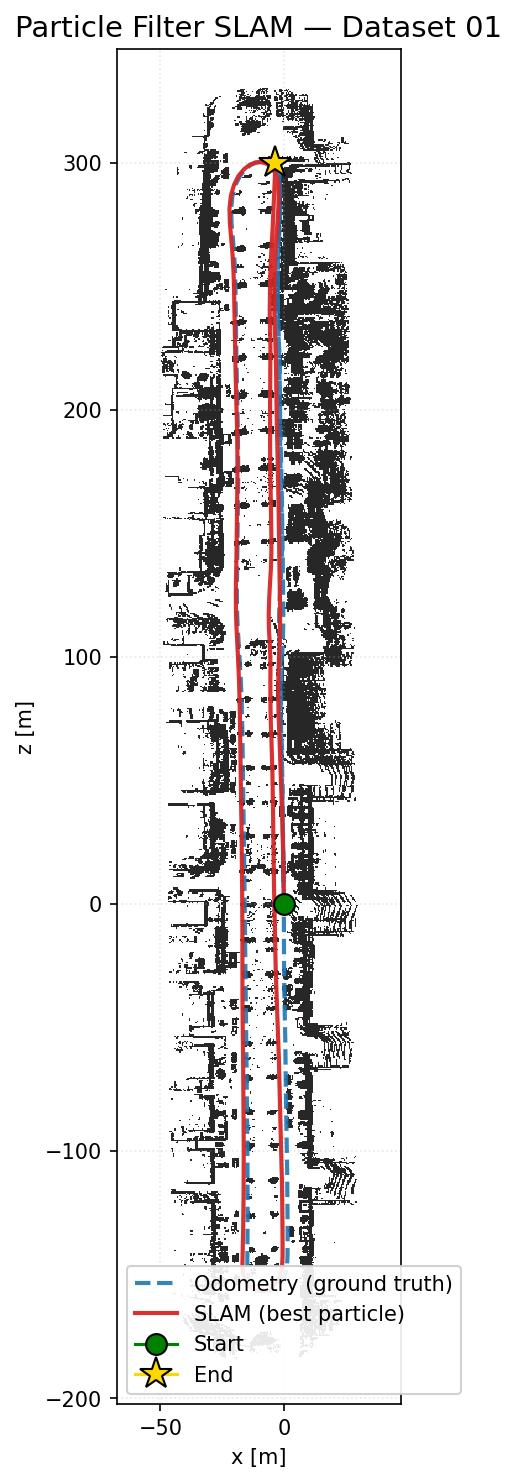
\includegraphics[width=0.45\textwidth]{../p2/logs/slam_01.jpg}
  \caption{Dataset 01 (KITTI seq.\ 06, 221 frames). A straight back-and-forth drive along a $\sim$500\,m boulevard; buildings on either side are mapped as parallel black strips. SLAM and odometry overlay almost perfectly, confirming the dynamics step on near-linear motion.}
  \label{fig:slam01}
\end{figure}

\begin{figure}[H]
  \centering
  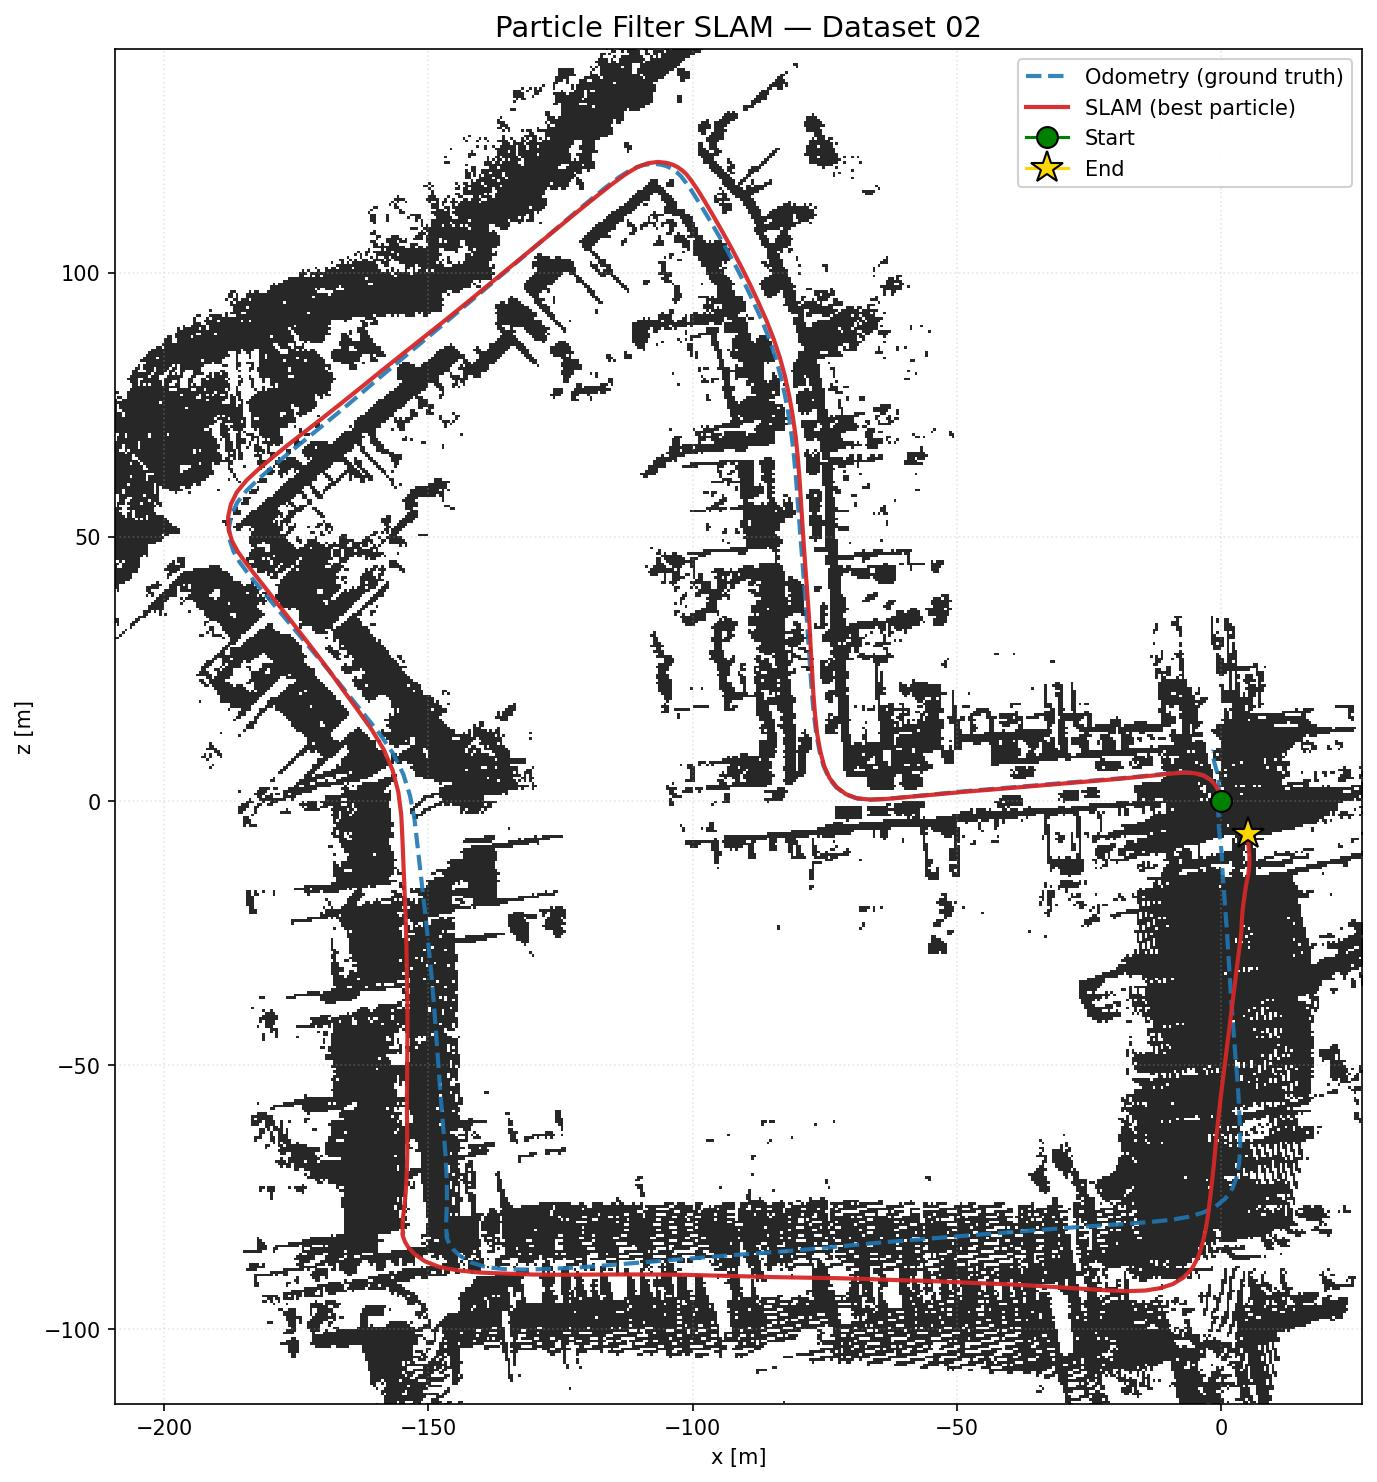
\includegraphics[width=0.75\textwidth]{../p2/logs/slam_02.jpg}
  \caption{Dataset 02 (KITTI seq.\ 07, 221 frames). A closed urban loop of $\sim$200\,m span, with clearly recognizable street networks and building blocks. SLAM tracks the odometry tightly through all four right-angle turns.}
  \label{fig:slam02}
\end{figure}

\begin{figure}[H]
  \centering
  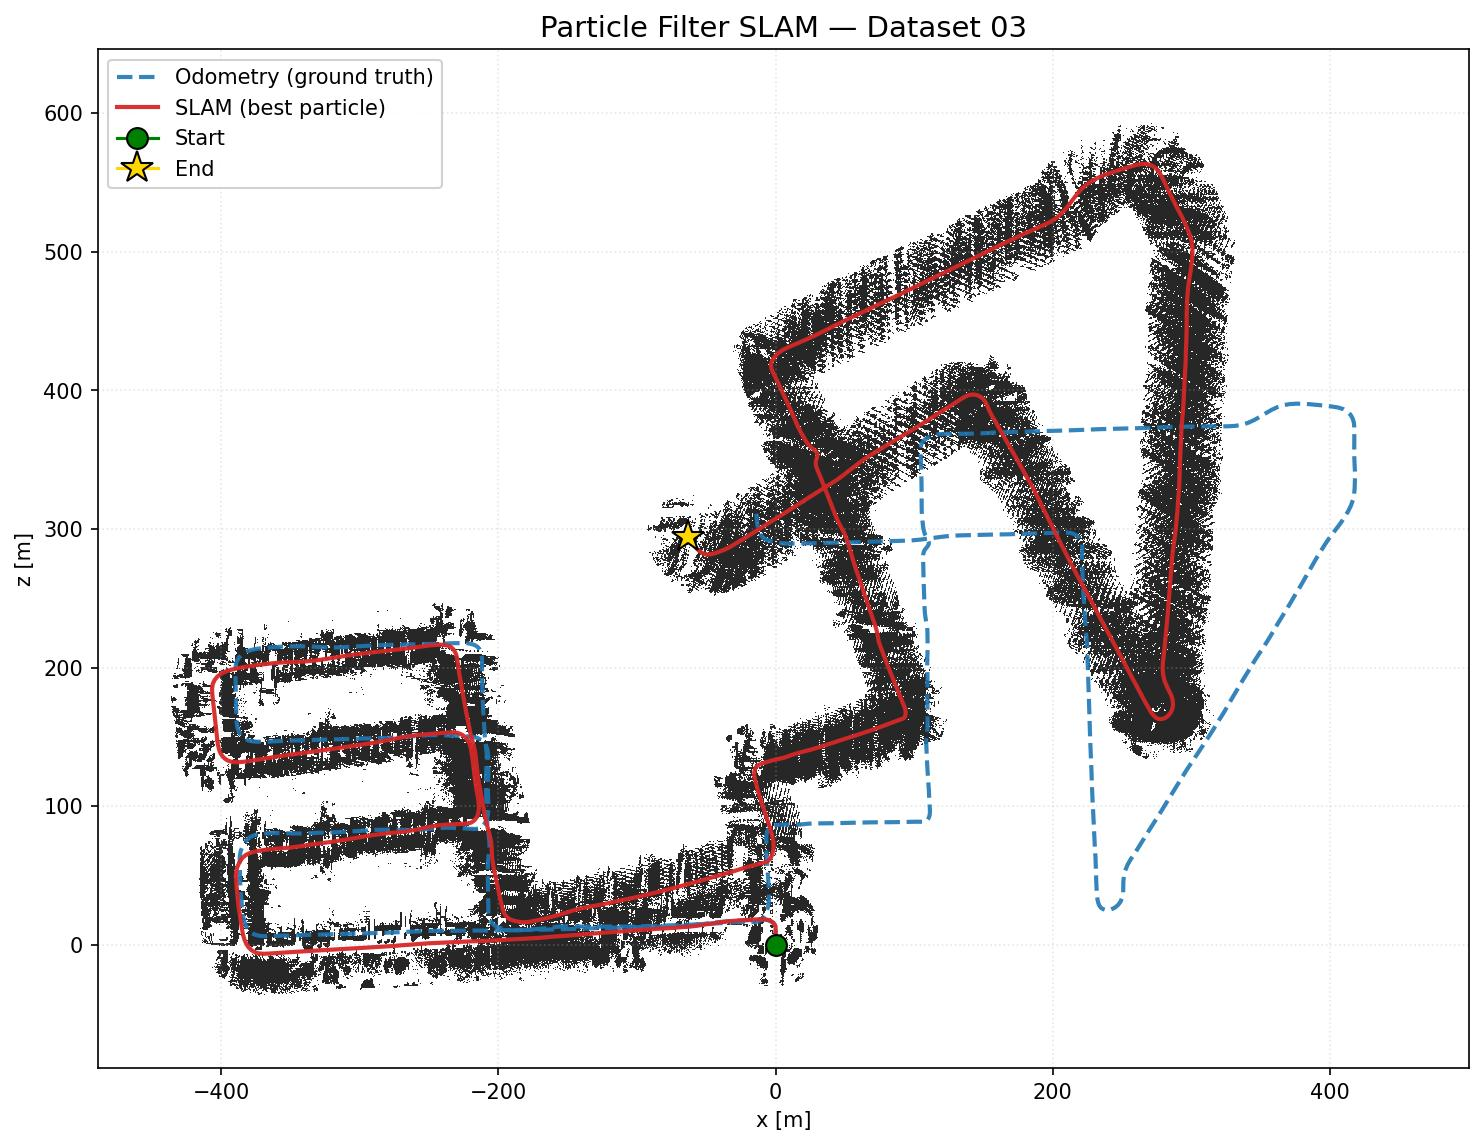
\includegraphics[width=0.78\textwidth]{../p2/logs/slam_03.jpg}
  \caption{Dataset 03 (KITTI seq.\ 08, 815 frames). The longest trajectory: a residential grid on the left, connected to a large highway-like loop on the right. The SLAM estimate (red) remains self-consistent with the map; the RTK odometry (blue dashed) on the right-hand loop diverges significantly from the mapped roadways, again showing poor GPS coverage in that region. The recovered map clearly shows parallel rows of buildings along each residential street.}
  \label{fig:slam03}
\end{figure}

\medskip
\noindent\textbf{Summary across datasets.}  The occupancy grid clearly recovers street geometry and building footprints on all four datasets. The SLAM trajectory matches the RTK odometry tightly on the short, structured sequences (01, 02); on the longer urban runs (00, 03) the RTK poses themselves show GPS artifacts in the far-from-start regions while the SLAM estimate remains aligned with the mapped road corridors.

\medskip
\noindent\textbf{Map parameters.}
Resolution $0.5$\,m/cell; bounds $x \in [-700, 700]$\,m, $z \in [-500, 900]$\,m; log-odds increments $\log 9 \approx 2.197$ (occupied), $-\log 9$ (free); occupancy threshold $P = 0.6$ (log-odds threshold $\approx 0.405$).

\medskip
\noindent\textbf{Point-cloud cleaning} (\texttt{clean\_point\_cloud}): keep points with reflectance $> 0.05$, height $\in (-1.0, 1.5)$\,m (relative to the LiDAR), and planar distance $< 30$\,m.  This removes ground returns, noise, and far-field sparse points which otherwise degrade the map.

\end{solution}

\clearpage
%% ============================================================
%% PROBLEM 3: NeRF
%% ============================================================
\begin{solution}[Building a NeRF]

\subsection*{(a) Data Loading and COLMAP}

We use the provided \texttt{transforms\_colmap.json} file which contains camera intrinsics and extrinsics for 100 LEGO images.

\medskip
\noindent\textbf{Camera parameters.}
The original images are $800 \times 800$.  We resize to $100 \times 100$ for efficient CPU training.  The focal length is computed from the horizontal FOV:
\[
  f_{\text{orig}} = \frac{W_{\text{orig}}}{2 \tan(\theta_x / 2)}, \qquad
  f = f_{\text{orig}} \times \frac{100}{800} = 138.89 \text{ px}.
\]
where $\theta_x$ = \texttt{camera\_angle\_x} from the JSON file.

After resizing: $H = 100$, $W = 100$, $f = 138.89$.

\subsection*{(b) Implementation of the NeRF}

We implement four key functions:

\medskip
\noindent\textbf{1. \texttt{get\_rays}$(H, W, f, T_w^c)$.}
For each pixel $(i,j)$, we compute the ray direction in camera coordinates using the pinhole model:
\[
  \mathbf{d}_{\text{cam}} = \left( \frac{j - W/2}{f}, \; -\frac{i - H/2}{f}, \; -1 \right).
\]
The NeRF coordinate convention is $+X$ right, $+Y$ up, $+Z$ back.  The ray direction and origin are transformed to world coordinates via the $4 \times 4$ camera-to-world matrix $T_w^c$:
\[
  \mathbf{o} = T_w^c[:3, 3], \qquad
  \mathbf{d} = \frac{R \cdot \mathbf{d}_{\text{cam}}}{\|R \cdot \mathbf{d}_{\text{cam}}\|}.
\]

\medskip
\noindent\textbf{2. \texttt{sample\_points\_from\_rays}.}
Given near bound $s_{\text{near}}$ and far bound $s_{\text{far}}$, we perform stratified sampling along each ray:
\[
  t_k = s_{\text{near}} + \frac{k}{N_{\text{sample}}} (s_{\text{far}} - s_{\text{near}}) + \xi_k, \quad \xi_k \sim \mathcal{U}\!\left(0, \frac{s_{\text{far}} - s_{\text{near}}}{N_{\text{sample}}}\right),
\]
yielding 3D sample points $\mathbf{x}_k = \mathbf{o} + t_k \mathbf{d}$.

\medskip
\noindent\textbf{3. \texttt{positional\_encoding}.}
We map 3D coordinates to a higher-dimensional space using sinusoidal functions:
\[
  \gamma(\mathbf{x}) = \bigl(\mathbf{x},\; \sin(2^0 \mathbf{x}),\, \cos(2^0 \mathbf{x}),\; \ldots,\; \sin(2^{L-1} \mathbf{x}),\, \cos(2^{L-1} \mathbf{x})\bigr)
\]
with $L = 10$ frequencies.  The output dimension is $(1 + 2 \times 10) \times 3 = 63$.

\medskip
\noindent\textbf{4. \texttt{volume\_rendering}.}
Given the predicted radiance field $(\sigma_k, \mathbf{c}_k)$ at each sample point (with $\sigma = \text{ReLU}(\cdot)$ and $\mathbf{c} = \text{sigmoid}(\cdot)$), we compute the rendered color via alpha compositing:
\begin{align}
  \delta_k &= t_{k+1} - t_k, \\
  \alpha_k &= 1 - e^{-\sigma_k \delta_k}, \\
  T_k &= \prod_{j=1}^{k-1}(1-\alpha_j), \\
  \hat{C} &= \sum_{k=1}^{N_{\text{sample}}} T_k \, \alpha_k \, \mathbf{c}_k.
\end{align}

\subsection*{(d) Network Training}

\noindent\textbf{Architecture.}
TinyNeRF: 4-layer MLP (Linear--ReLU--Linear--ReLU--Linear--ReLU--Linear), input dimension 63 (positional encoding), hidden dimension $h_{\text{dim}} = 32$, output dimension 4 (RGB + $\sigma$).  Total parameters: 4,292.

\medskip
\noindent\textbf{Hyperparameters.}
\begin{itemize}
  \item $N_{\text{sample}} = 32$, $h_{\text{dim}} = 32$
  \item $s_{\text{near}} = 2.0$, $s_{\text{far}} = 6.0$
  \item Learning rate: $5 \times 10^{-3}$ (Adam)
  \item Training iterations: 1000
  \item Image resolution: $100 \times 100$
\end{itemize}

\begin{figure}[H]
  \centering
  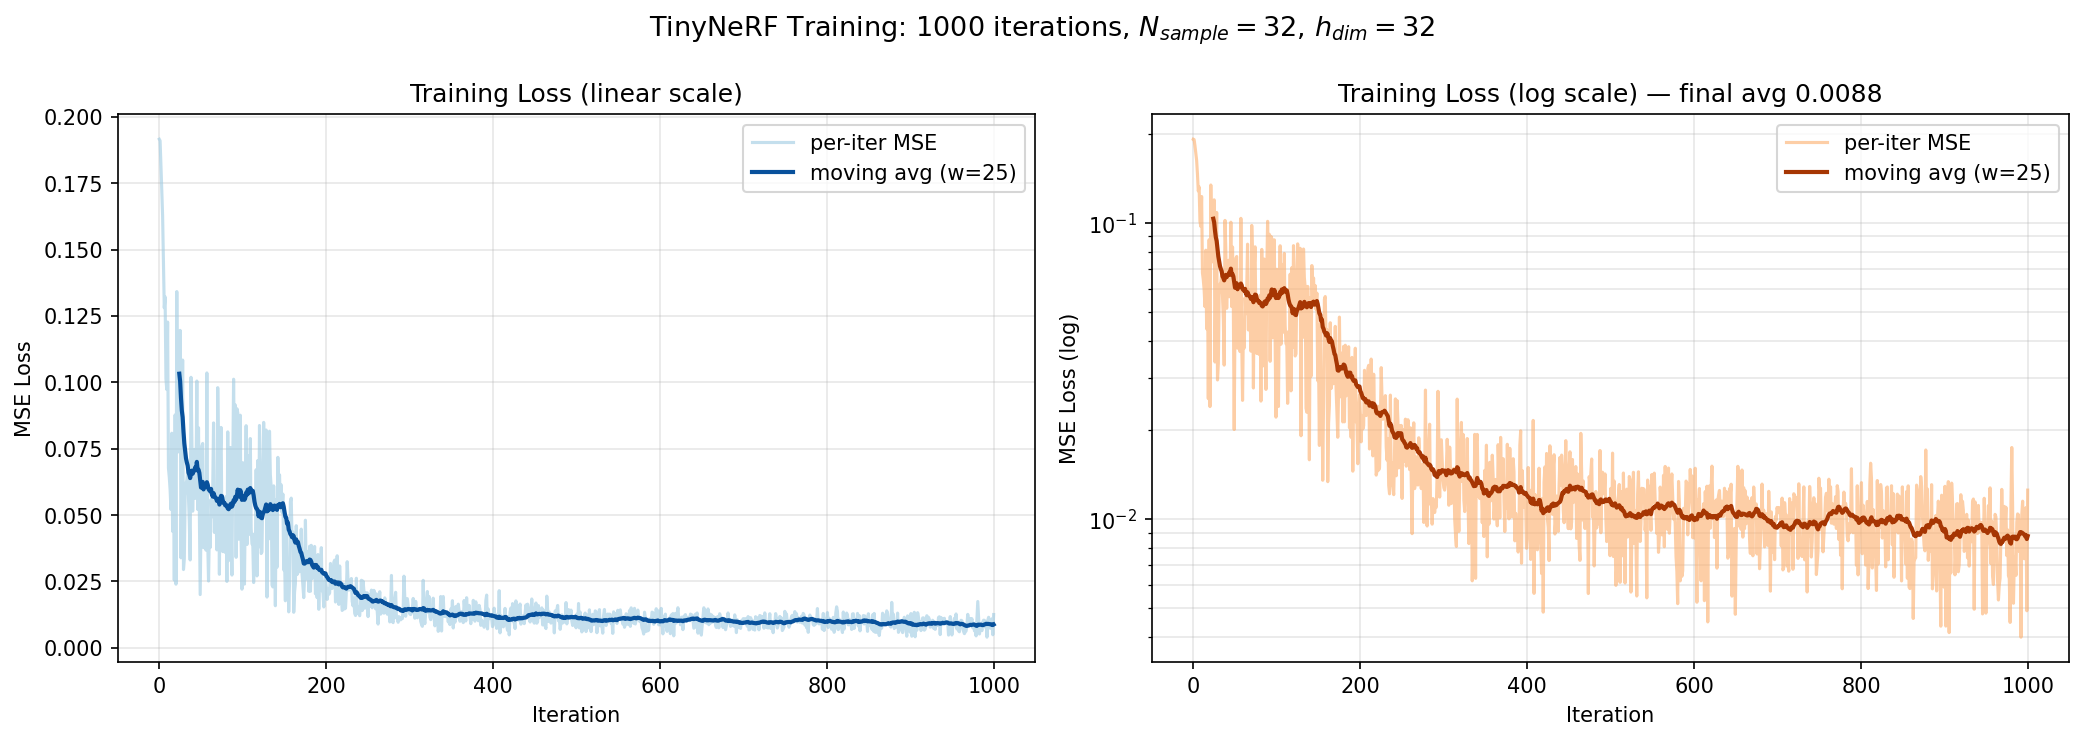
\includegraphics[width=0.7\textwidth]{../p3/training_loss.png}
  \caption{Training loss (MSE) vs.\ iteration, shown in linear (left) and log (right) scale with a moving-average overlay (window 25). The smoothed loss drops from $\approx 0.20$ at iter 0 to a final $\approx 0.0088$ at iter 1000, at which point the NeRF recovers the overall object shape but remains blurry (expected for TinyNeRF with $h_{\text{dim}}=32$ on CPU).}
  \label{fig:nerf_loss}
\end{figure}

\begin{figure}[H]
  \centering
  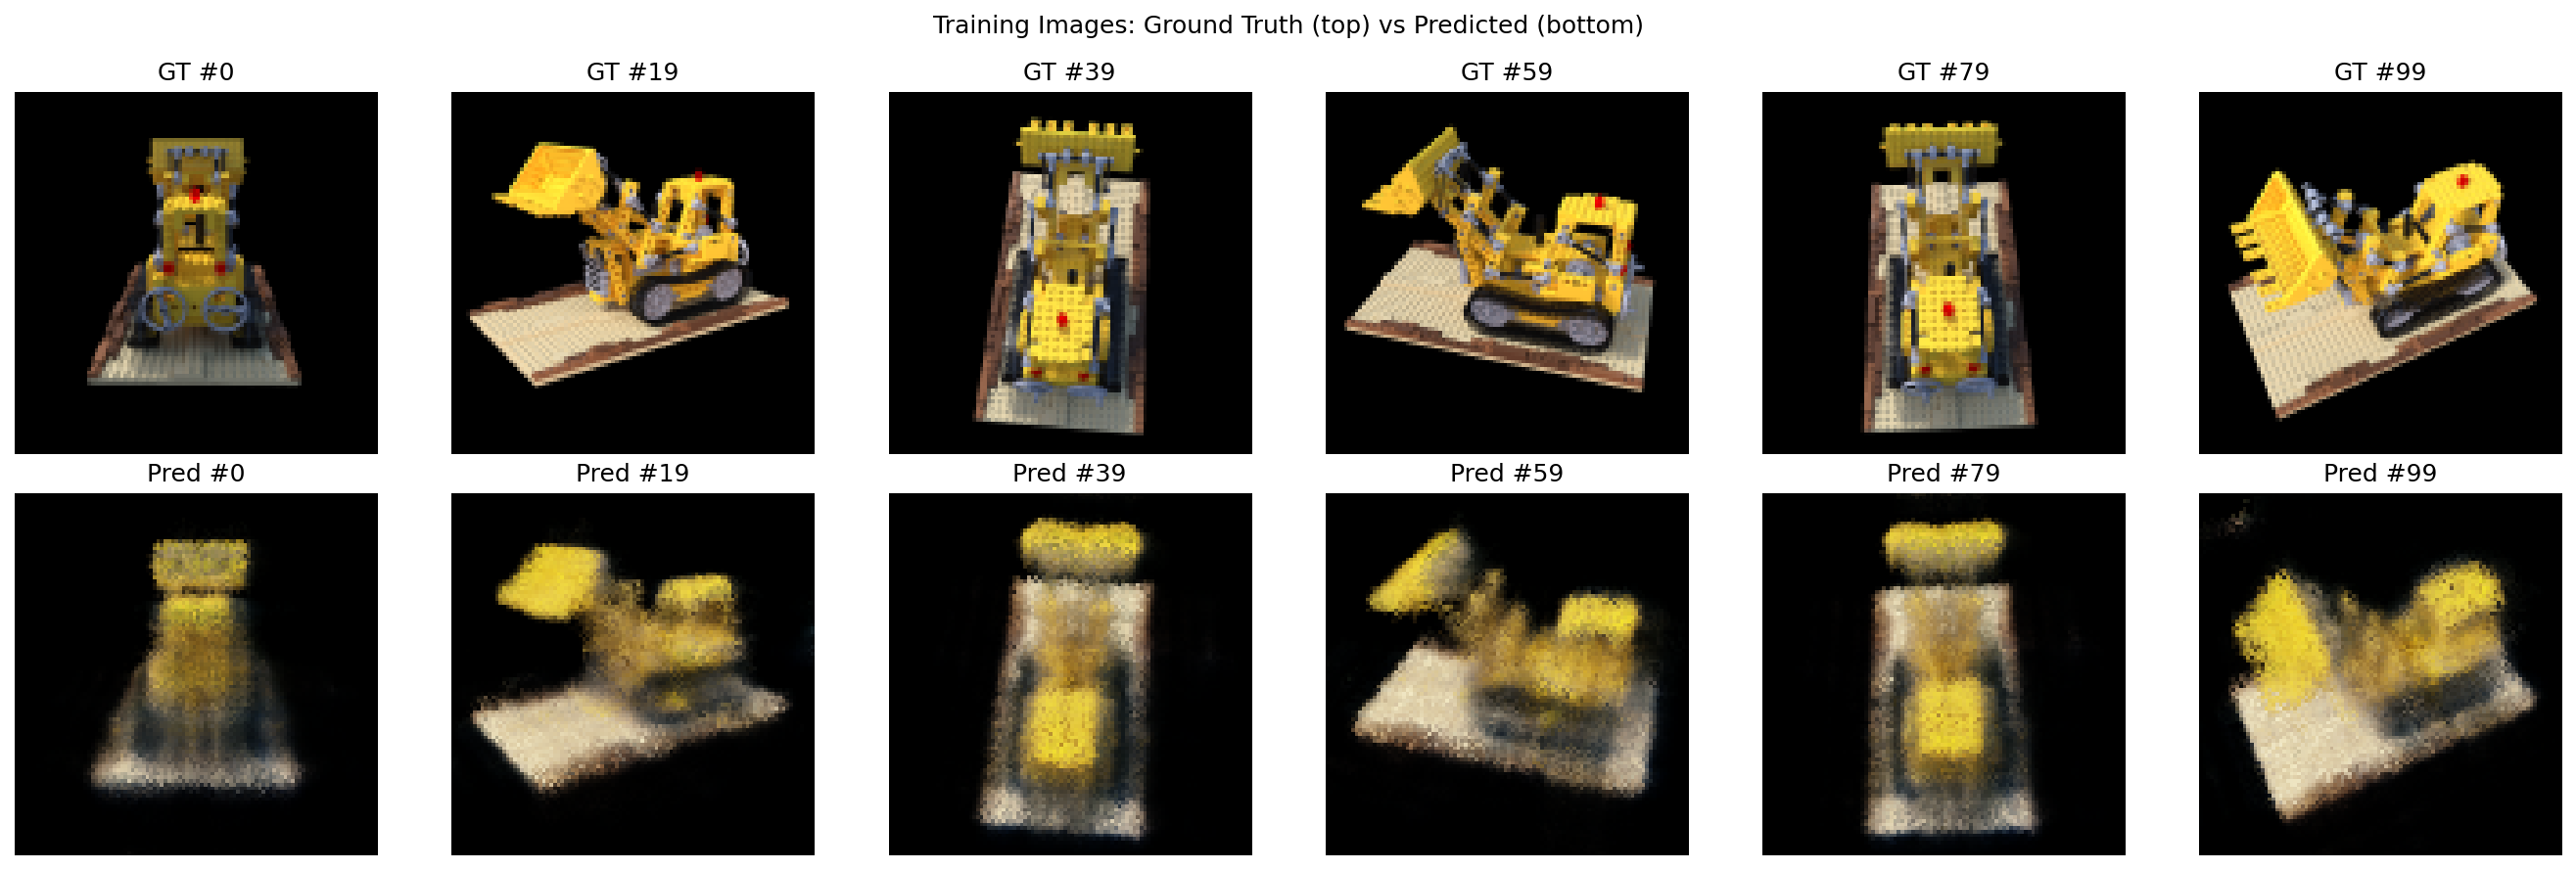
\includegraphics[width=0.95\textwidth]{../p3/training_comparison.png}
  \caption{Training set comparison: ground truth (top) vs.\ NeRF prediction (bottom) for 6 sampled viewpoints.}
  \label{fig:nerf_train}
\end{figure}

\subsection*{(e) Inference}

\begin{figure}[H]
  \centering
  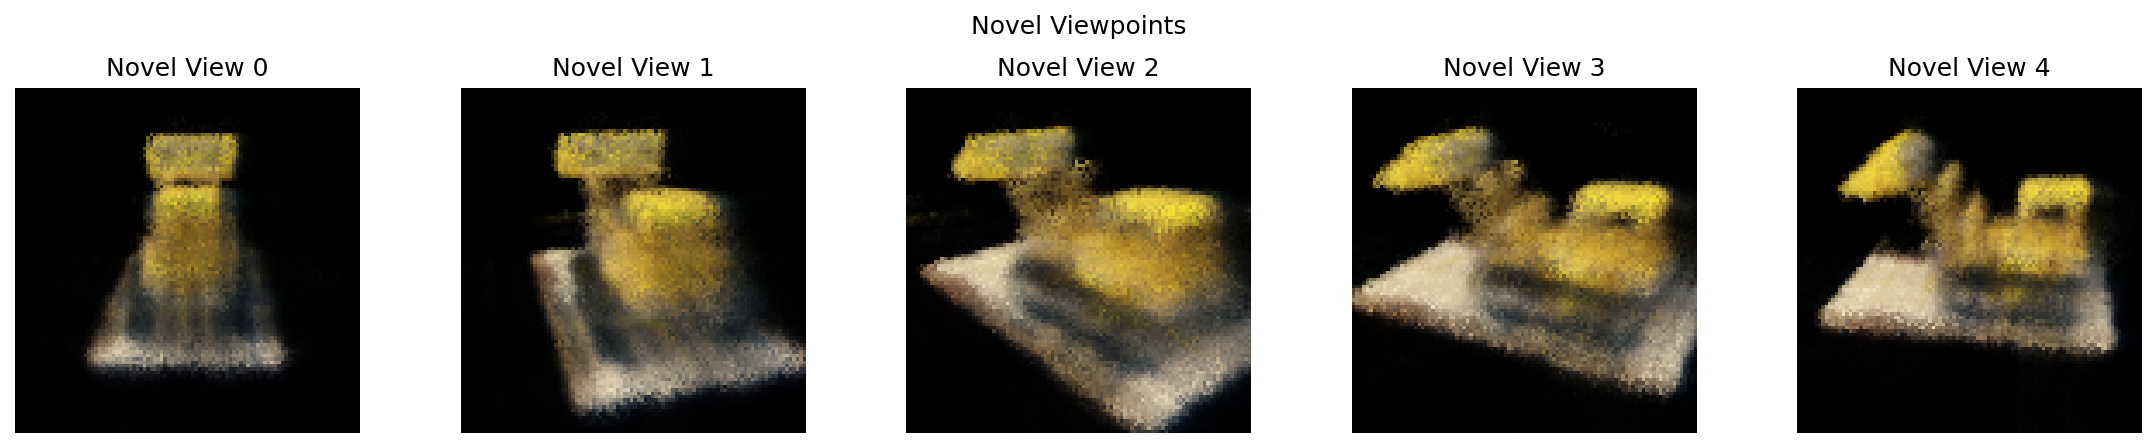
\includegraphics[width=0.95\textwidth]{../p3/novel_views.png}
  \caption{Novel viewpoint rendering: 5 interpolated poses between training views.}
  \label{fig:nerf_novel}
\end{figure}

Novel views are generated by linearly interpolating between two training poses.  The NeRF produces coherent geometry from nearby viewpoints, but may show artifacts (blurriness, color drift) for poses far from the training distribution, which is expected given the simplified architecture and limited training.

\end{solution}

\end{document}
